\section{Durchführung}
\label{sec:Durchführung}
In Abbildung \ref{fig:aufbau} ist der Schematische Aufbau der verwendeten Apperatur wiedergegeben. 
Mit dieser Apperatur wird sowohl die Messung mit einseitiger, als auch die mit beidseitiger Einspannung durchgeführt.
Des weiteren werden vier Proben zur Vermessung benötigt. Dabei handelt es sich um zwei runde und zwei rechteckige Stäbe, von denen zunächst das Gewicht sowie die Maße vermessen werden.
\begin{figure}
    \centering
    \caption{Schematische Darstellung einer Apperatur zur Vermessung elastisch gebogener Stäbe \cite{v103}}
    \label{fig:aufbau}
    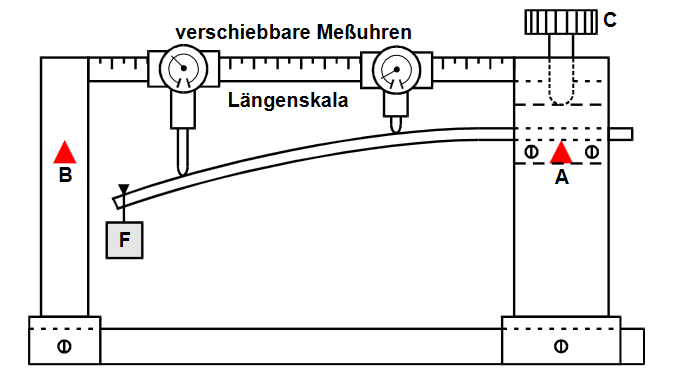
\includegraphics[width=0.5\textwidth]{pics/aufbau.png}
\end{figure}
Für den ersten Versuchsteil wird ein Probestab an der Stelle $x=\SI{0}{\centi\metre}$ einseitig eingespannt. Eine verschiebbaren Messuhr wird an der Stelle $x=\SI{5}{\centi\metre}$ auf null tariert. Danach wird das Gewicht der Masse $M=\SI{}{\gram}$ an der
Stelle $x=\SI{53}{\centi\metre}$ befestigt und die Differenz wird an der Messuhr abgelesen. Bei runden Stäben ist darauf zu achten, dass die Messuhr oben auf dem Stab drauf ist.
Danach wird das Gewicht entfernt und die Messuhr wird um $\SI{5}{\centi\metre}$ verschoben. Es erfolgt eine erneute Messung der Differenz. Das Verfahren wird wiederholt bis die Messuhr in etwa bei 
$\SI{50}{\centi\metre}$ ist und dann für den nächsten Stab auch wieder durchgeführt.
Für den zweiten Messteil wird ein Probestab beidseitig aufgelegt. Dabei wird eine Seite eingespannt und die andere nur aufgelegt. Dieses mal werden zwei Messuhren verwendet, wobei die erste sich an der Stelle $x=\SI{5}{\centi\metre}$ und die zweite an der Stelle
$x \approx \SI{50}{\centi\metre}$ befindet. Es werden erneut die Uhren auf null tariert, sodass, nachdem das Gewicht $M=\SI{}{\gram}$ in die Mitte angebracht wurde, die Differenz einfach abgelesen werden kann.
Danach werden die Uhren um jeweils $\SI{5}{\centi\metre}$ aufeinander zu geschoben und die Messung wird wiederholt. Dieses Verfahren wird durchgeführt bis zehn Messwerte entnommen wurden und dann wird es für alle anderen Stäbe wiederholt.
